\chapter{Core Knowledge}\label{cap:planificación}

\section{Introducción}

There are currently numerous techniques used in artificial intelligence. These not only come from physics or mathematics, but are also closely related to economics and computer science. Such is the catalog of possibilities available to us that it is often difficult to keep up to date, as new ideas emerge every day. Therefore, in order to obtain a better general understanding of this work, we will explain the principles of some of the methods or techniques used in the project, since understanding them will make it easier to follow the workflow. 
s
\section{Neural Networks}

If we look at the history of science and technology, we can observe that many advances are inspired by real biological systems. For example, a camera shares many similarities with the human eye. Another example is the processor, which consists of a large number of transistors connected to perform calculations. Neural networks are also part of this trend, as their structure is approximately based on biological neural networks. For this reason, we will briefly introduce this concept before discussing artificial neural networks.

\subsection{Neurons}

Biologically speaking, a neuron is the smallest unit of the nervous system, responsible for receiving, processing and transmitting information through electrical impulses. They have three main components:

\begin{itemize}
    \item The cell body or soma contains the nucleus and the organelles necessary for the correct functioning of the neuron. All signals received by the neuron via the dendrites are transmitted to this section. If the sum of these signals exceeds a certain threshold in the axon cone, a new electrical impulse is generated in response and propagated along the axon. This area is specialised in this task, thanks to its high concentration of sodium. As the number of connections between neurons increases, they become faster, allowing us to think faster, i.e. certain tasks take less time. This process, in which one neuron transmits information to another, is called a synapse.
    \item Dendrites are branched extensions of the soma that receive electrical signals from other neurons and convey them toward the cell body.
    \item The axon is a long projection that extends from the soma, typically originating at the axon hillock, toward the synaptic terminals. Its main function is to transmit electrical impulses from the cell body to other neurons, muscles, or glands.
    \item Synaptic terminals have many branches, each one finishes on a synaptic button. These structures are the responsible for releasing the electric signal to other cells.
\end{itemize}

\begin{figure}[h!]
    \centering
    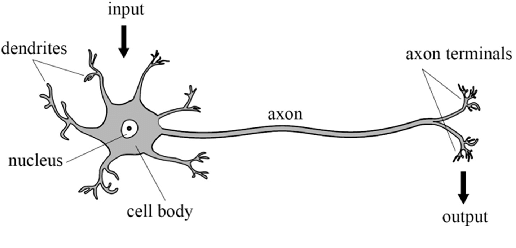
\includegraphics[width=0.6\textwidth]{figures/neural_parts.png}
    \caption{Parts of a neuron. Source: \cite{partsNeuron}}
    \label{fig:neuron}
\end{figure}

\subsection{Virtual neural networks}

Understanding the origin of neural networks can be crucial to improving our methodology. Since we already know what a neural network is, we will now introduce its virtual counterpart. As we discuss artificial neural networks, we will compare them with their biological equivalents to deepen our understanding of the topic. The goal is to become aware that the differences between them are not as significant as they may seem.

\subsubsection{Simple perceptron}

The simple perceptron is one of the most basic models of an artificial neural network. It functions similarly to a biological neuron. It receives multiple inputs, each multiplied by an associated weight, sums them, and then applies an activation function, typically a threshold or sigmoid function. In the case of the threshold function, if the weighted sum of the inputs exceeds a certain threshold, the perceptron outputs a signal (usually 1); otherwise, it does not (usually 0). 

Since this process resembles the biological one, we can think of it as follows: the neuron receives information (inputs), which is transmitted toward the nucleus, analogous to the activation function in artificial neurons, and, if the signal is strong enough, the neuron emits a new signal, similar to the output of the activation function.

\begin{figure}[h!]
    \centering
    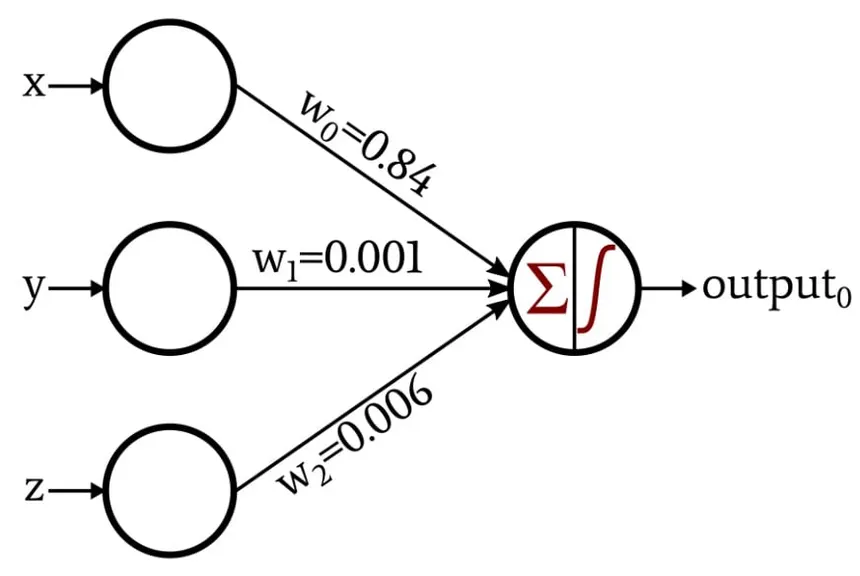
\includegraphics[width=0.6\textwidth]{figures/simple_perceptron.png}
    \caption{Simple perceptron. Source: \cite{simplePerceptron}}
    \label{fig:simplePerceptron}
\end{figure}

Having established how the perceptron functions conceptually, it is now appropriate to introduce its mathematical foundation. Analyzing how the perceptron transforms data in the input space (typically a plane in two dimensions) can provide valuable insights for designing more effective neural network architectures.

\section{Predictions trees}


\section{Shap values}